%http://freshmeat.net/articles/view/667/
\documentclass[mcgill,slideColor,colorBG,pdf]{prosper}
\usepackage{epsfig, pstricks, graphicx, alltt, fancyvrb, qtree, ulem}

\title{Optimizing Compilers with the Soot - Eclipse Plugin}
\author{Jennifer Lhot\'ak\\
Sable Research Group\\
McGill University\\
\  \\
\  \\
\  \\
This work is sponsored in part by an IBM Eclipse Innovation Grant and NSERC.\\
}

\begin{document}
\maketitle

\begin{slide} {Introduction}
\begin{itemize}
\item Topic: introduction to optimizing compilers
\item Target: people with some knowledge of compilers
\end{itemize}
\end{slide}

\begin{slide} {Outline}
\begin{itemize}
\item Introduction 
\item Structure
\item Intermediate Representations
\item Control Flow Analysis
\item Data Flow Analysis
\end{itemize}
\end{slide}

\begin{slide} {Introduction - Components}
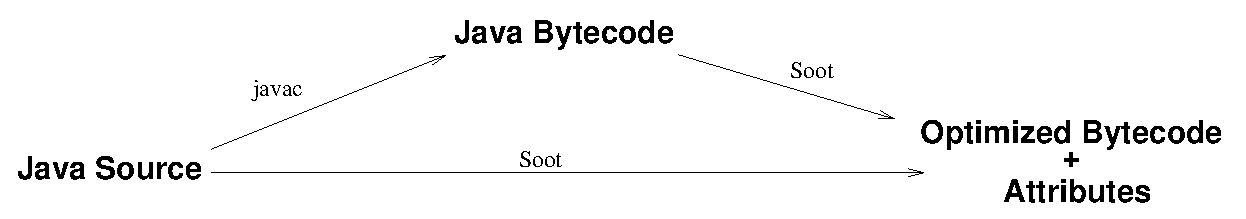
\epsfig{file=components.eps,width=4.3in}
\end{slide}

\begin{slide} {Introduction - Virtual Machines}
\begin{itemize}
\item AOT (ahead-of-time) - can take a long time 
\item JIT (just-in-time) - has to be fast
\item JITopt - compiler is slower but code is faster
\end{itemize}
\end{slide}

\begin{slide} {Introduction - Effective Optimizations}
\begin{itemize}
\item apply optimization to correct IR
\item design analysis to statically determine program properties
\item use analysis results to perform transformation
\end{itemize}
\end{slide}


\begin{slide} {Introduction - Where To Optimize?}
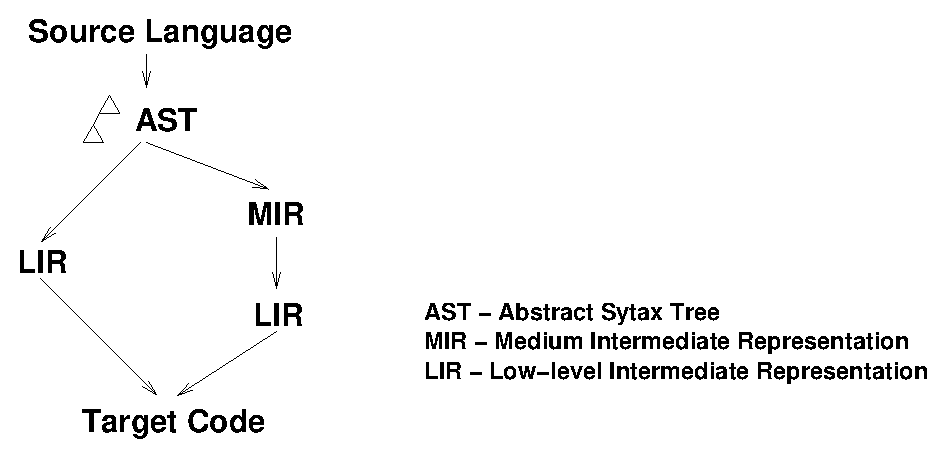
\epsfig{file=where_to_opt.eps,width=4.3in}
\end{slide}

\begin{slide} {Introduction - Performance}
\begin{itemize}
\item should work across many programs
\item should affect key parts of the program
\item should use "efficient-enough" algorithms
\end{itemize}
90\% of time spent in inner loops or commonly called methods!
\end{slide}

\begin{slide} {Introduction - Loop Invariant Exercise}
\begin{itemize}
\item switch To Eclipse
\item run Soot on the \texttt{LoopInvariant.java} sample code
\begin{itemize}
\item right click on file in Package Explorer
\item select Soot - Process Source File - Run Soot ...
\end{itemize}
\item enable the Loop Invariant Tagger
\begin{itemize}
\item select Phase Options - Jimple Annotation Pack - Loop Invariant Tagger
\item check the Enable box
\end{itemize}
\end{itemize}
\end{slide}

\begin{slide} {Introduction - Exercise Notes}
\begin{itemize}
\item the loop invariant expression $y = x + z$ is highlighted in red
\item mouse over to see the "is loop invariant" tooltip
\item notice the expression $y = x + i$ is not highlighted (depends on loop index)
\item the constant $j = 1$ is loop invariant
\item the expression $m = j + 1$ which uses a constant and a constant local is loop invariant
\end{itemize}
\end{slide}

\begin{slide} {Introduction - Loop Invariants}
An expression is loop invariant if:
\begin{itemize}
\item operands are all constants
\item or operands have reaching definitions only from outside the loop body
\end{itemize}
\end{slide}

\begin{slide} {Introduction - Forwards/Backwards Analyses}
Forwards Analysis:
\begin{itemize}
\item use information about the past
\item propagate information forward
\end{itemize}
Backwards Analysis:
\begin{itemize}
\item use information about the future
\item propagate information backwards
\end{itemize}
\end{slide}

\begin{slide} {Introduction - Reaching Defs Exercise}
\begin{itemize}
\item switch To Eclipse
\item run Soot on the \texttt{ReachingDefs.java} sample code
\begin{itemize}
\item right click on file in Package Explorer
\item select Soot - Process Source File - Run Soot ...
\end{itemize}
\item enable the Reaching Defs Tagger
\begin{itemize}
\item select Phase Options - Jimple Annotation Pack - Reaching Defs Tagger
\item check the Enable box
\end{itemize}
\end{itemize}

\end{slide}

\begin{slide} {Introduction - Exercise Notes}
\begin{itemize}
\item the expressions $j = x + y$, $x = x + 1$ and $z = x + 2$ have SootAttribute icons

\epsfig{file=sa.eps,width=3mm} 
in margin
\item mouse over the statements to see the list of reaching defs
\item click icon to get list of reaching defs
\item select reaching def from list to navigate to definition statement
\end{itemize}
\end{slide}

\begin{slide} {Introduction - Reaching Defs}
A definition statement is a reaching definition if it could be the most recent definition of some variable used in the current statement % need better reaching def definition
\begin{itemize}
\item forwards analysis
\end{itemize}
\end{slide}

\begin{slide} {Introduction - Live Variables Exercise}
\begin{itemize}
\item switch To Eclipse
\item run Soot on the \texttt{Liveness.java} sample code
\begin{itemize}
\item right click on file in Package Explorer
\item select Soot - Process Source File - Run Soot ...
\end{itemize}
\item enable the Live Variables Tagger
\begin{itemize}
\item select Phase Options - Jimple Annotation Pack - Live Variables Tagger
\item check the Enable box
\end{itemize}
\end{itemize}

\end{slide}

\begin{slide} {Introduction - Exercise Notes}
\begin{itemize}
\item the variables highlighted in green are live at that point in the program
\item mouse over the statements to see the live variable tooltips
\end{itemize}
\end{slide}

\begin{slide} {Introduction - Live Variable}
A variable is live if at some point in the future the variable will be used again % need better definition
\begin{itemize}
\item backwards analysis
\item sample use: register allocation
\end{itemize}
\end{slide}

\begin{slide} {Introduction - Live Variables Exercise 2}
\begin{itemize}
\item switch To Eclipse
\item run Soot on the \texttt{LiveInteractive.java} sample code
\begin{itemize}
\item right click on file in Package Explorer
\item select Soot - Process Source File - Run Soot ...
\end{itemize}
\end{itemize}

\end{slide}

\begin{slide} {Introduction - Live Variables Excercise 2 cont.}
\begin{itemize}
\item enable the Interaction and the Live Variables Tagger
\begin{itemize}
\item under General Options check Interactive Mode 
\item select Output Options - under Output Options select Jimple
\item select Phase Options - Jimple Annotation Pack - Live Variables Tagger
\item check the Enable box
\end{itemize}
\end{itemize}
\end{slide}

\begin{slide} {Introduction - Exercise Notes}
\begin{itemize}
\item the control flow graph is displayed in the editor
\item use the Step Forward button
\epsfig{file=step_forward.eps,width=3mm}
to see the analysis as it is being generated
\end{itemize}
\end{slide}

\begin{slide} {Structure of Compilers - Frontend}
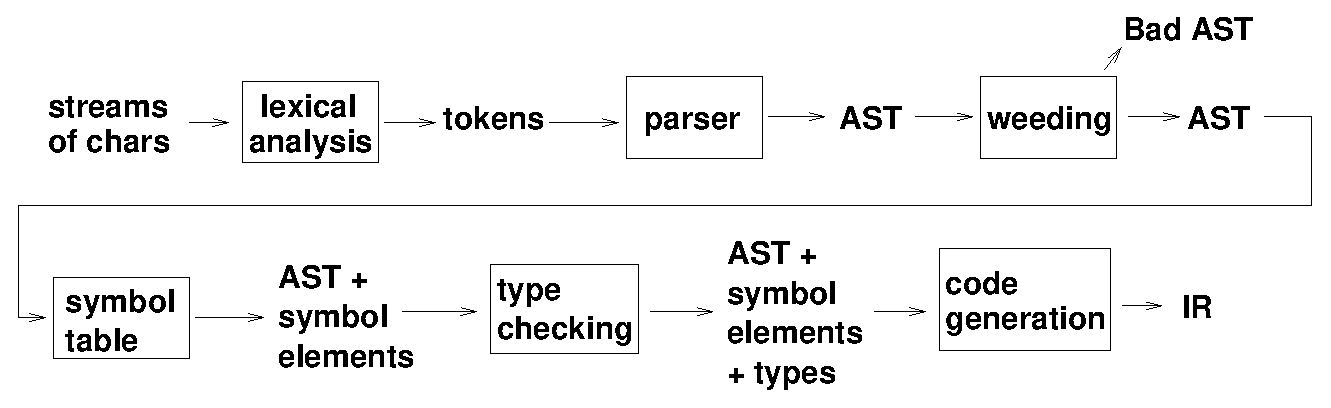
\epsfig{file=frontend_struc.eps,width=4in}
\end{slide}

\begin{slide} {Structure of Compilers - Backend}
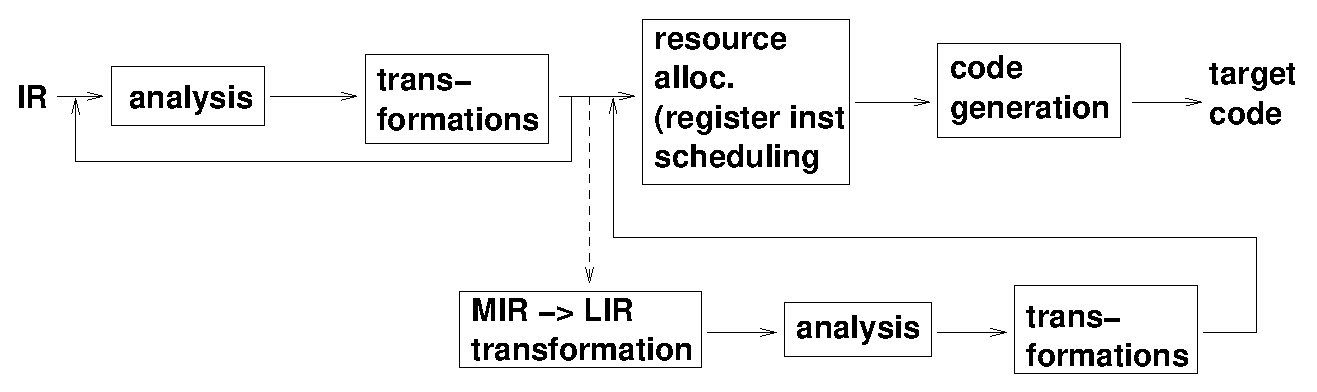
\epsfig{file=backend_struc.eps,width=4in}
\end{slide}

\begin{slide} {Structure of Compilers - Java Systems}
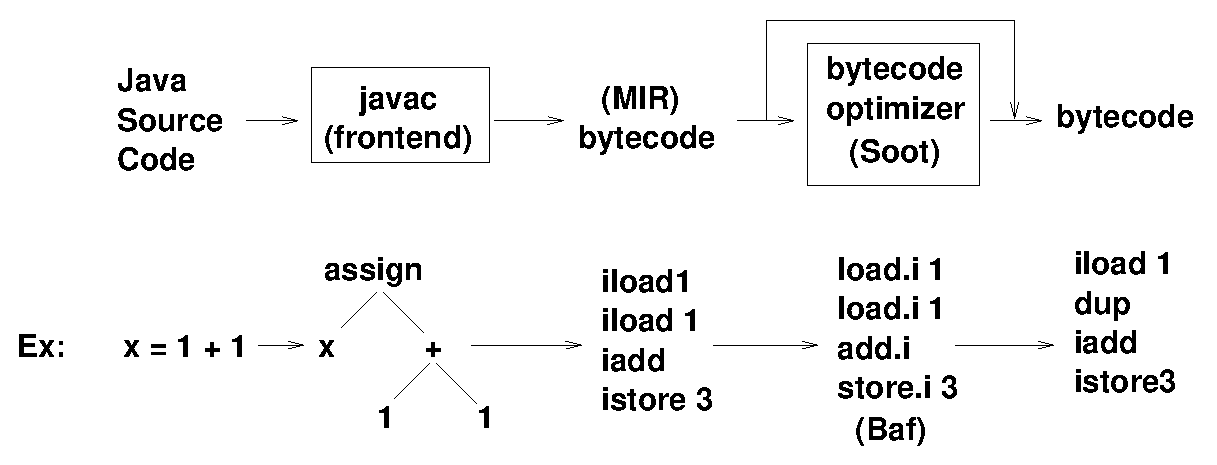
\epsfig{file=java_struc.eps,width=4in}
\end{slide}

\begin{slide} {Intermediate Representations}
$$n\left\{ \begin{array}{c} Pascal\\C\\Fortran\\Java\\ML\\Scheme\\AspectJ \end{array} \rightarrow \fbox{IR} \rightarrow \begin{array}{c} x86\\Sparc\\Mips\\68000\\Cray\\Smp \end{array}\right\} m$$
\end{slide}

\begin{slide} {Intermediate Representations - Need Many}
\begin{itemize}
\item need enough info about high-level program (ex: types)
\item need to be close enough to low-level architecture (for low-level optimization opportunities)
\item use family of IRs (high, medium, low)
\end{itemize}
\end{slide}

\begin{slide} {Intermediate Representations - Design}
\begin{itemize}
\item designing IRs is an art
\item dependent on kinds of optimizations
\item some optimizations are difficult on some IRs
\begin{itemize}
\item ex: transformations difficult on stack-based IR
\end{itemize}
\end{itemize}
\end{slide}

\begin{slide} {Intermediate Representations - High-Level}
\begin{itemize}
\item used in early stages (front-end)
\item AST based or graph based (ex: Grimp in Soot)
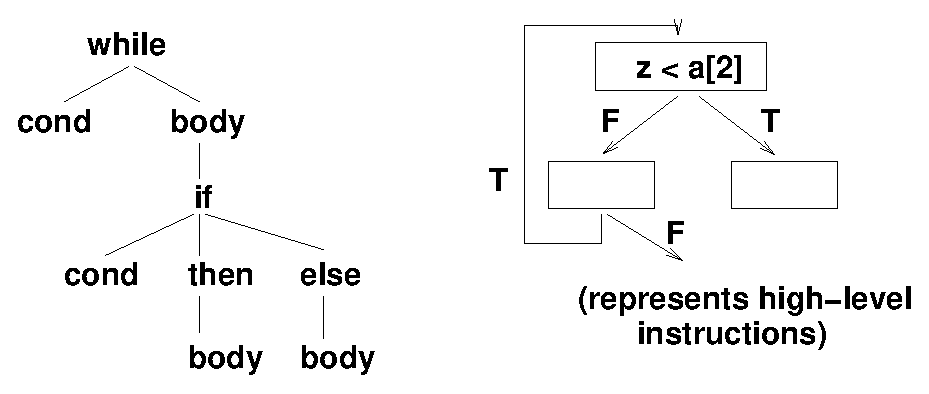
\epsfig{file=highlevel.eps,width=4in}
\end{itemize}
\end{slide}

\begin{slide} {Intermediate Representations - Grimp Exercise}
\begin{itemize}
\item switch to Eclipse
\item run Soot on the \texttt{GrimpExample.java} sample code
\begin{itemize}
\item right click on file in Package Explorer
\item select Soot - Process Source File - Create Grimp ...
\end{itemize}
\item view generated Grimp
\begin{itemize}
\item expand sootOutput folder
\item open \texttt{GrimpExample.grimp} file
\end{itemize}
\end{itemize}
\end{slide}

\begin{slide} {Intermediate Representations - Exercise Notes}
\begin{itemize}
\item notice the high-level expression in the if statement $if$ $x <a[\$i0]$
\item notice the expression $x = x + a[4] + 2$ is all in one statement
\end{itemize}
\end{slide}

\begin{slide} {Intermediate Representations - Medium-Level}
\begin{itemize}
\item somewhat language independent
\item represent variables from program and temps
\item only 1 operation per statement
\item most analyses and transformations are at this level
\end{itemize}
\end{slide}

\begin{slide} {Intermediate Representations - Jimple Exercise}
\begin{itemize}
\item switch to Eclipse
\item run Soot on the \texttt{JimpleExample.java} sample code
\begin{itemize}
\item right click on file in Package Explorer
\item select Soot - Process Source File - Create Jimple ...
\end{itemize}
\item view generated Jimple
\begin{itemize}
\item expand sootOutput folder
\item open \texttt{JimpleExample.jimple} file
\end{itemize}
\end{itemize}
\end{slide}

\begin{slide} {Intermediate Representations - Exercise Notes}
\begin{itemize}
\item notice the expression in the if statement $if$ $x < \$i3$ and the array access is done in a previous statement
\item notice the expression $x = x + a[4] + 2$ has been split into three statements
\end{itemize}
\end{slide}

\begin{slide} {Intermediate Representations - Low-Level}
\begin{itemize}
\item correspond closely to target machine
\item allow maximum low-level optimizations
\item make machine resources explicit
\begin{itemize}
\item registers
\item delay slots
\item instructions
\end{itemize}
\end{itemize}
\end{slide}

\begin{slide} {Control Flow Analysis - Find Control Structure}
\begin{enumerate}
\item basic blocks (straight line code)
\begin{itemize}
\item good for local analysis
\end{itemize}
\item extended basic blocks
\begin{itemize}
\item good for instruction scheduling
\end{itemize}
\item loops/recursive cycles
\begin{itemize}
\item important for optimizations
\end{itemize}
\item reducible (well-structured)
\begin{itemize}
\item inexpensive analysis
\end{itemize}

\end{enumerate}
\end{slide}

\begin{slide} {Control Flow Analysis - 3-addr Statements}
\begin{itemize}
\item Simple:
\begin{itemize}
\item x $\leftarrow$ y op z
\item x $\leftarrow$ op y
\item x $\leftarrow$ y
\item goto L
\item if x relop y goto L
\end{itemize}
\item Procedure Calls:
\begin{itemize}
\item foo(a, z)
\item x $\leftarrow$ foo(a, z)
\end{itemize}
\end{itemize}
\end{slide}

\begin{slide} {Control Flow Analysis - 3-addr Statements}
\begin{itemize}
\item Pointers:
\begin{itemize}
\item x $\leftarrow$ addr y 
\item x $\leftarrow$ * y
\item * y $\leftarrow$ x
\item x $\leftarrow$ * y.f
\item * y.f $\leftarrow$ x
\end{itemize}
\item Arrays:
\begin{itemize}
\item x $\leftarrow$ a[i]
\item a[i] $\leftarrow$ x
\end{itemize}
\end{itemize}
\end{slide}

\begin{slide} {Control Flow Analysis - Finding Basic Blocks}
\begin{enumerate}
\item Determine set of leaders (first statement of basic block)
\begin{itemize}
\item first statement of sequence
\item statements that are targets of gotos
\item statements following gotos
\end{itemize}
\item for each leader its basic block consists of the leader and all statements up to the next leader
\item add control flow edges between basic blocks
\end{enumerate}
\end{slide}

\begin{slide} {Control Flow Analysis - Finding BB Example}
\begin{tiny}
$$
\begin{array}{c}
a \leftarrow 1\\
b \leftarrow 3\\
d \leftarrow a + b\\
L1: if a < b goto L2\\
a \leftarrow a - 1\\
goto L3\\
L2: a \leftarrow a + 1\\
b \leftarrow b - 1\\
if a < b goto L2\\
L3: d \leftarrow a + b\\
if d > 0 goto L1\\
print (d)
\end{array}
$$
\end{tiny}
\end{slide}

\begin{slide} {Control Flow Analysis - Leaders - First Statement}
\begin{tiny}
$$
\begin{array}{c}
{\red \fbox{a $\leftarrow$ 1}}\\
b \leftarrow 3\\
d \leftarrow a + b\\
L1: if a < b goto L2\\
a \leftarrow a - 1\\
goto L3\\
L2: a \leftarrow a + 1\\
b \leftarrow b - 1\\
if a < b goto L2\\
L3: d \leftarrow a + b\\
if d > 0 goto L1\\
print (d)
\end{array}
$$
\end{tiny}
\end{slide}

\begin{slide} {Control Flow Analysis - Leaders - Goto Targets}
\begin{tiny}
$$
\begin{array}{c}
{\blue \fbox{a $\leftarrow$ 1}}\\
b \leftarrow 3\\
d \leftarrow a + b\\
{\red \fbox{L1: if a < b goto L2}}\\
a \leftarrow a - 1\\
goto L3\\
{\red \fbox{L2: a $\leftarrow$ a + 1}}\\
b \leftarrow b - 1\\
if a < b goto L2\\
{\red \fbox{L3: d $\leftarrow$ a + b}}\\
if d > 0 goto L1\\
print (d)
\end{array}
$$
\end{tiny}
\end{slide}

\begin{slide} {Control Flow Analysis - Leaders - Follow Gotos}
\begin{tiny}
$$
\begin{array}{c}
{\blue \fbox{a $\leftarrow$ 1}}\\
b \leftarrow 3\\
d \leftarrow a + b\\
{\blue \fbox{L1: if a < b goto L2}}\\
{\red \fbox{a $\leftarrow$ a - 1}}\\
goto L3\\
{\blue \fbox{L2: a $\leftarrow$ a + 1}}\\
b \leftarrow b - 1\\
if a < b goto L2\\
{\blue \fbox{L3: d $\leftarrow$ a + b}}\\
if d > 0 goto L1\\
{\red \fbox{print (d)}}
\end{array}
$$
\end{tiny}
\end{slide}

\begin{slide} {Control Flow Analysis - Find Basic Blocks}
\begin{tiny}
$$
\begin{array}{c}
\fbox{\begin{tabular}{c}{\blue \fbox{a $\leftarrow$ 1}}\\
b $\leftarrow$ 3\\
d $\leftarrow$ a + b \end{tabular}}\\
\fbox{{\blue \fbox{L1: if a < b goto L2}}}\\
\fbox{\begin{tabular}{c}{\blue \fbox{a $\leftarrow$ a - 1}}\\
goto L3 \end{tabular}}\\
\fbox{\begin{tabular}{c}{\blue \fbox{L2: a $\leftarrow$ a + 1}}\\
b $\leftarrow$ b - 1\\
if a < b goto L2 \end{tabular}}\\
\fbox{\begin{tabular}{c}{\blue \fbox{L3: d $\leftarrow$ a + b}}\\
if d > 0 goto L1\end{tabular}}\\
\fbox{{\blue \fbox{print (d)}}}
\end{array}
$$
\end{tiny}
\end{slide}

\begin{slide} {Control Flow Analysis - Add Edges}
\begin{center}
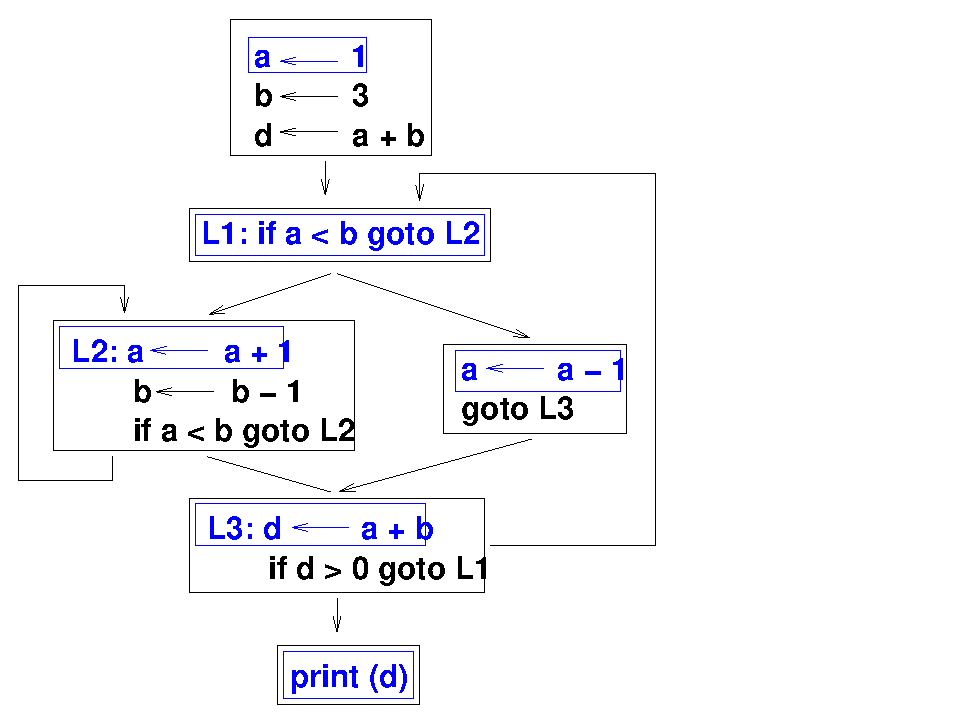
\epsfig{file=basic_blocks.eps,width=4in}
\end{center}
\end{slide}

\begin{slide} {Control Flow Analysis - Irreducible}
A graph is irreducible if it has a pattern like:
\begin{center}
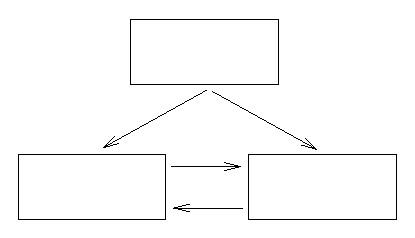
\epsfig{file=irreducible.eps,width=2in}
\end{center}
\end{slide}

\begin{slide} {Control Flow Analysis - Extended Basic Blocks}
Extended basic blocks: a maximal set of instructions beginning with leader that contains no join nodes
\end{slide}

\begin{slide} {Control Flow Analysis - Loops}
\begin{itemize}
\item Explicit Loops (AST)\\ 
\begin{center}
\textbf{while} (<cond>) <body>
\end{center}
\item Implicit Loops (CFG)
\end{itemize}
\begin{center}
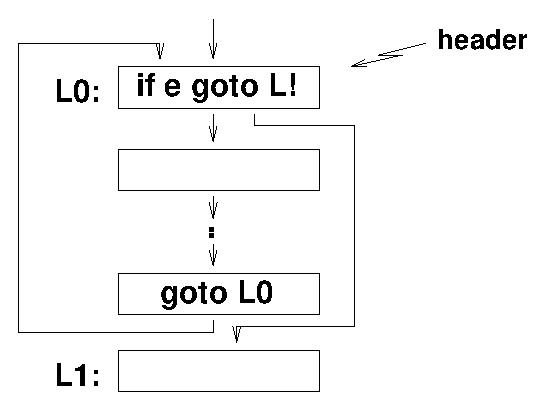
\epsfig{file=implicit_loop.eps,width=2in}
\end{center}
\end{slide}

\begin{slide} {Control Flow Analysis - Loops}
A loop (single entrance, multi-exit) in a cfg is a set of nodes S including a header node h with the following properties
\begin{itemize}
\item from any node in S there is a path of directed edges to h 
\item there is a path of directed edges from h to any node in S
\item there is no edge from any node outside S to any node inside S except for h
\end{itemize}
\end{slide}

\begin{slide} {Control Flow Analysis - Loops}
Single entry, multi exit loop:\\
\ \\
\begin{center}
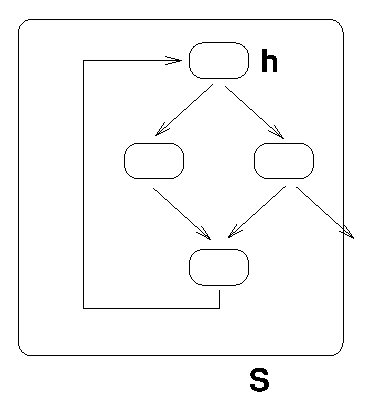
\epsfig{file=loop.eps,width=1.6in}
\end{center}
\end{slide}

\begin{slide} {Control Flow Analysis - Loops}
Loops:
\begin{center}
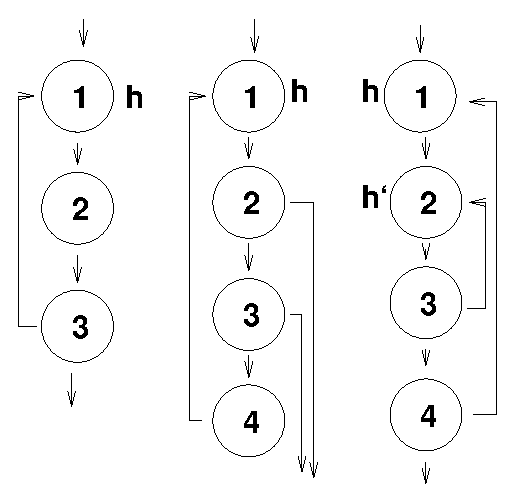
\epsfig{file=loops.eps,width=1.3in}
\end{center}
Not Loops (irreducible): 
\begin{center}
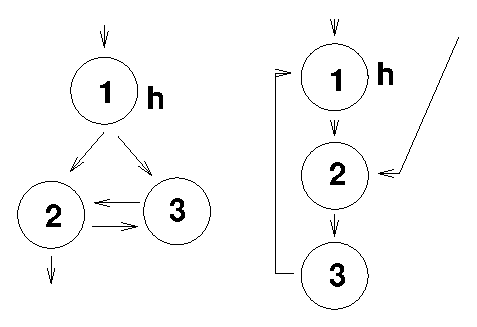
\epsfig{file=not_loops.eps,width=1.3in}
\end{center}
\end{slide}

\begin{slide} {Control Flow Analysis - Reducible Flow Graphs}
\begin{itemize}
\item only get reducible flow graphs in Java and C (without gotos)
\item dataflow analysis can be done on reducible flow graphs
\end{itemize}
\end{slide}

\begin{slide} {Control Flow Analysis - How to Find Loops}
\begin{itemize}
\item need dominators
\begin{center}
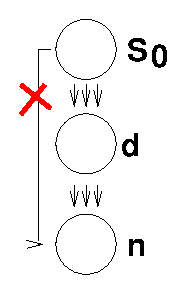
\epsfig{file=dominators_simple.eps,height=1in}
\end{center}
\item a node d dominates a node n if every path of directed edges from $S_0$ to n must go through d
\item every node dominates itself
\end{itemize}
\end{slide}

\begin{slide} {Control Flow Analysis - How to Find Loops Cont.}
\begin{center}
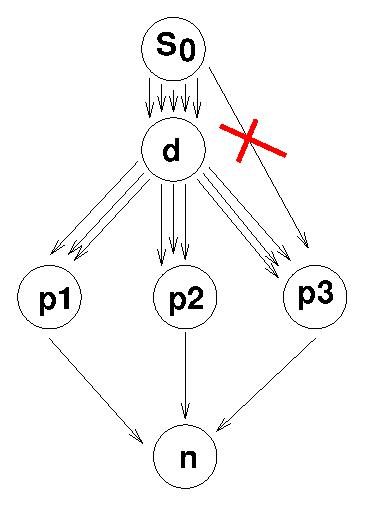
\epsfig{file=dominators_complex.eps,height=1.4in}
\end{center}
\begin{itemize}
\item $D(n) = \{n\} U (\cap_{p \in pred[n]} D[p])$
\item solve flow equations - start with full sets
\end{itemize}
\end{slide}

\begin{slide} {Control Flow Analysis - Dominators Exercise}
\begin{itemize}
\item switch to Eclipse
\item run Soot on the \texttt{DominatorExample.java} sample code
\begin{itemize}
\item right click on file in Package Explorer
\item select Soot - Process Source File - Run Soot ...
\end{itemize}
\end{itemize}
\end{slide}


\begin{slide} {Control Flow Analysis - Dominators Exercise}
\begin{itemize}
\item output Jimple
\begin{itemize}
\item select Output Options - Output Format - Jimple File
\end{itemize}
\item enable the Dominators Tagger
\begin{itemize}
\item select Phase Options - Jimple Annotation Pack - Dominators Tagger
\item check the Enable box
\end{itemize}
\end{itemize}
\end{slide}

\begin{slide} {Control Flow Analysis - Exercise Notes}
\begin{itemize}
\item click on the SootAttribute icon

\epsfig{file=sa.eps,width=3mm} 
in the margin of a statement to see a list of dominators - select one to navigate to the dominator
\item open the \texttt{sootOutput/DominatorExample.jimple} file to explore the dominators within the Jimple IR
\end{itemize}
\end{slide}

\begin{slide} {Control Flow Analysis - Immediate Dominators}
d dominates n and e dominates n $\Rightarrow$ \\d dominates e or e dominates d\\
\ \\
\begin{center}
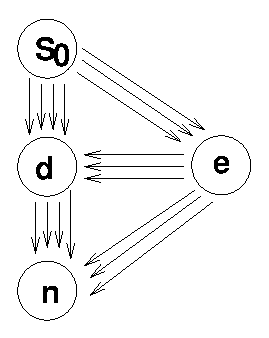
\epsfig{file=dominators_imm.eps,height=1.4in}
\end{center}
\end{slide}

\begin{slide} {Control Flow Analysis - Immediate Dominators}
Every node n has no more than one immediate dominator, idom(n) such that:
\begin{enumerate}
\item idom(n) is not the same as n
\item idom(n) dominates n
\item idom(n) does not dominate any other dominator of n
\end{enumerate}
\begin{center}
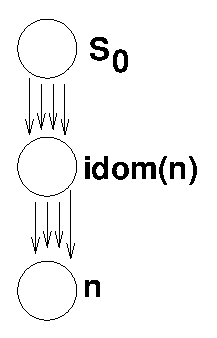
\epsfig{file=idom.eps,height=1in}
\end{center}
\end{slide}

\begin{slide} {Control Flow Analysis - Natural Loops}
Given an edge n $\rightarrow$ h:
\begin{itemize}
\item h dominates n
\item all x such that h dominates x and $\exists$ a path x $\rightarrow$ n which does not contain h
\begin{center}
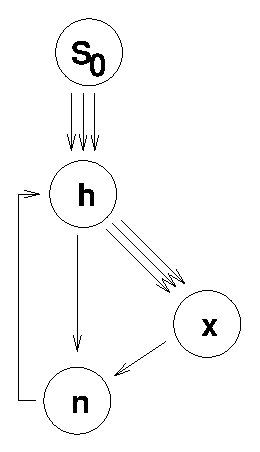
\epsfig{file=natural_loops.eps,height=1in}
\end{center}
\item continue is not a natural loop
\end{itemize}
\end{slide}

\begin{slide} {Control Flow Analysis - Dominator Trees}
\begin{itemize}
\item use every node in a cfg
\item add edges for idoms
\begin{center}
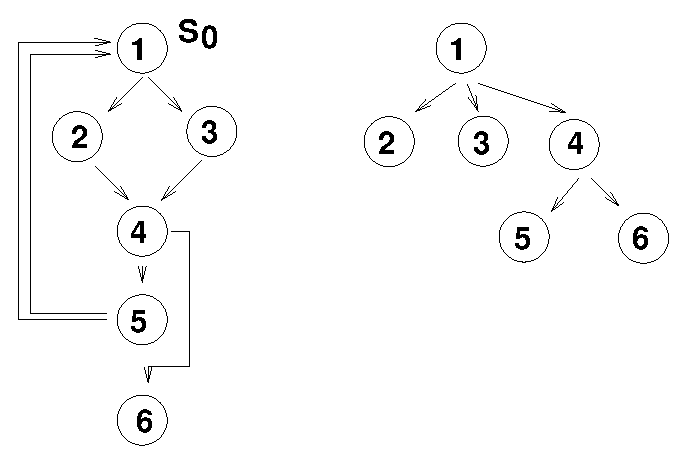
\epsfig{file=dom_tree.eps,height=1in}
\end{center}
\item cfg edge from n to h such that h dominates n is a back-edge (5 $\rightarrow$ 1 (1 dominates 5))
\item for each back-edge there is a sub-graph that is a loop
\end{itemize}
\end{slide}


\begin{slide} {Data Flow Analysis}
\begin{itemize}
\item Local: within basic blocks
\item Global/Intra-procedural: on one control flow graph for a method (at call to another method make worst case assumptions)
\item Inter-procedural: hook up all control flow graphs for all methods 
\begin{itemize}
\item hard for dynamic linking
\item long / big difficult
\end{itemize}
\end{itemize}
\end{slide}

\begin{slide} {Data Flow Analysis - Steps}
\begin{enumerate}
\item figure out what you're computing
\begin{itemize}
\item ex: set of variables live at each statement
\end{itemize}
\item precisely define what it is you're computing
\begin{itemize}
\item ex: a variable v is live at program point p if $\exists$ a path from p to the end of the program on which there is a use of v
\end{itemize}
\item decide whether the analysis is forwards or backwards
\begin{itemize}
\item ex: backwards
\end{itemize}
\end{enumerate}
\end{slide}

\begin{slide} {Data Flow Analysis - Steps}
\begin{enumerate}
\item[4.] decide which merge operator to use
\begin{itemize}
\item ex: union
\end{itemize}
\item[5.] define flow equations $in(s) = f(out(s))$
\begin{itemize}
\item ex: $S: z = x + y $\\
$defs(S) = \{z\}$ and $uses(S) = \{x, y\}$\\
$in(S) = (out(S) - defs(S)) U uses(S)$\\
       $= (out(S) U uses(S)) - defs(S) ->$ is incorrect consider $z = z - 1$  

\end{itemize}
\end{enumerate}
\end{slide}

\begin{slide} {Data Flow Analysis - Steps}
\begin{enumerate}
\item[6.] determine value of start or end node 
\begin{itemize}
\item ex: \{\}
\end{itemize}
\item[7.] determine approximation to use for all the sets initially
\begin{itemize}
\item ex: \{\} - (least safe)
\end{itemize}
\end{enumerate}
\end{slide}

\begin{slide} {Data Flow Analysis - Standard Approach}
\begin{center}
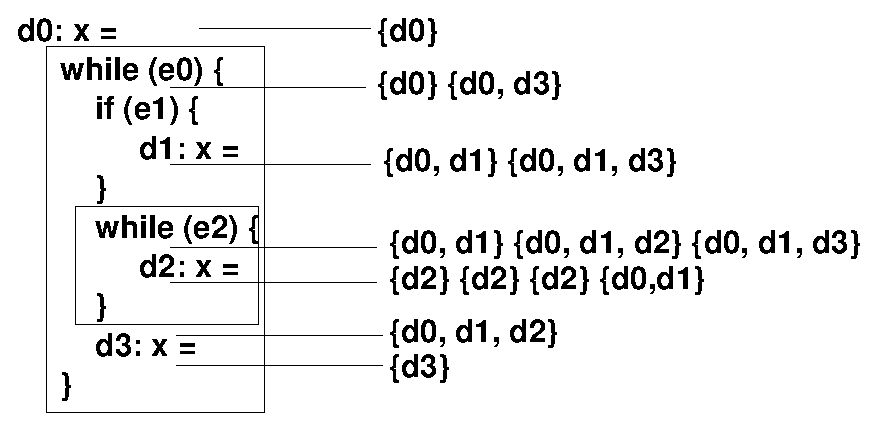
\epsfig{file=standard.eps,width=4in}
\end{center}
For loop nesting of n - $2^n$ iterations
\end{slide}

\begin{slide} {Data Flow Analysis - Structure Based Approach}
\begin{enumerate}
\item compute gen and kill sets from bottom-up and store in AST
\item proceed top-down
\begin{itemize}
\item compute output for S
\item compute outputs for sub-structures of S
\end{itemize}
\end{enumerate}
\begin{tiny}
\Tree [.while e [.body [.$S_1$ [.if $S_i$ $S_j$ ] ] $S_2$ $S_3$ ] ]
\end{tiny}
\end{slide}

\begin{slide} {Data Flow Analysis - Worklist Method}
\begin{itemize}
\item put all blocks on worklist (order matters) 
\item initialize in
\item choose $B_x$ to start
\end{itemize}
\begin{center}
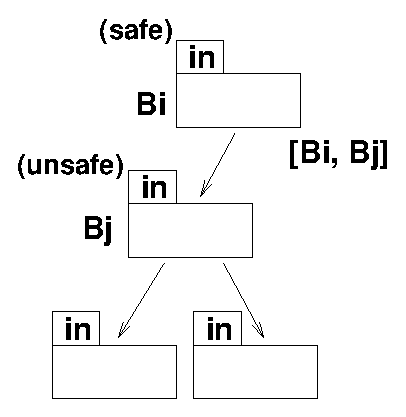
\epsfig{file=worklist.eps,width=1.7in}
\end{center}
\end{slide}

\begin{slide} {Data Flow Analysis - Iterative Method}
Algorithm:
\begin{tiny}
\begin{Verbatim}[commandchars=\\\{\}]
for each block B do         {\blue // assume in[B] = \{\}}
    out[B] = gen[B]

repeat 
    change = false
    for each block B do     {\blue // in depth-first order}
        begin
            in[B] = \(\cup_{P \in{pred of B}}\) out[P]
            oldout = out[B]
            out[B] = gen[B] \(\cup\) (in[B] - kill[B])
            if out[B] <> oldout then change = true
         end
until not change  
\end{Verbatim}
\end{tiny}
\end{slide}

\begin{slide} {Data Flow Analysis - Iterative Method}
\begin{center}
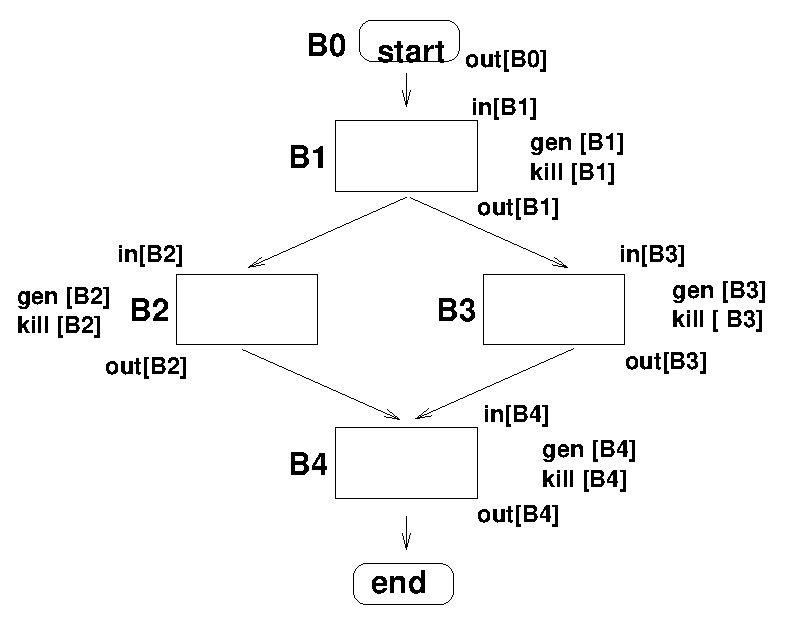
\epsfig{file=iterative.eps,height=2.5in}
\end{center}
\end{slide}

\begin{slide} {Data Flow Analysis - One Iteration?}
\begin{center}
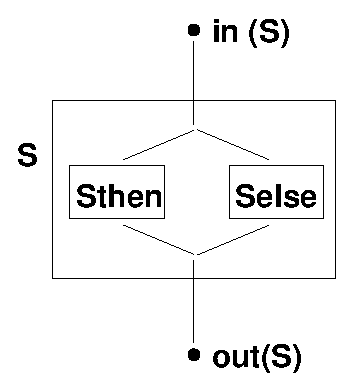
\epsfig{file=one_iteration1.eps,height=1.5in}
\end{center}
\ \\
$out(S) = gen(S) \cup (in(S) - kill(S))$\\
$gen(S) = gen(Sthen) \cup gen(Selse)$\\
$kill(S) = kill(Sthen) \cap kill(Selse)$
\end{slide}

\begin{slide} {Data Flow Analysis - One Iteration?}
\begin{center}
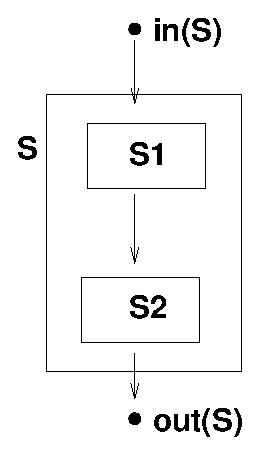
\epsfig{file=one_iteration2.eps,height=1.5in}
\end{center}
\ \\
$gen(S) = gen(S2) \cup (gen(S1) - kill(S2))$\\
$kill(S) = kill(S2) \cup (kill(S1) - gen(S2)$
\end{slide}

\begin{slide} {Data Flow Analysis - One Iteration?}
\texttt{while} (e) body
\begin{center}
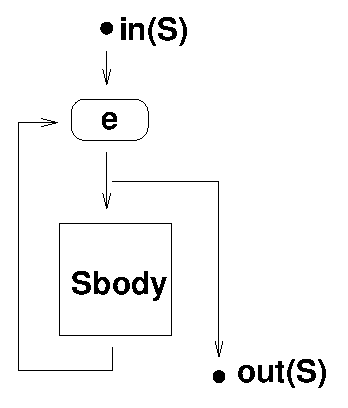
\epsfig{file=one_iteration3.eps,height=1.5in}
\end{center}
\ \\
$out(S) = in(S) \bowtie gen(Sbody) \cup (in(S) - kill(Sbody))$\\
$gen(S) = gen(Sbody)$\\
$kill(S) = \{\}$
\end{slide}

\begin{slide} {Data Flow Analysis - One Iteration?}
\texttt{do} body \texttt{while} (e)
\begin{center}
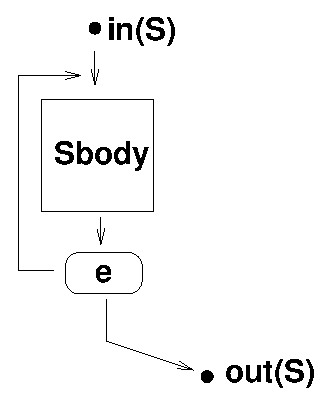
\epsfig{file=one_iteration4.eps,height=1.5in}
\end{center}
\ \\
\begin{tiny}
$out(S) = gen(Sbody) \cup (in(S) \cup out(S) - kill(Sbody))$\\
$out(S)_0 = \{\}$\\
$out(S)_1 = gen(Sbody) \cup (in(S) - kill(Sbody)$\\
$out(S)_2 = gen(Sbody) \cup (in(S) \cup [ gen(Sbody) \cup (in(S) - kill(Sbody)] - kill(Sbody)) = gen(Sbody) \cup (in(S) - kill(Sbody))$
\end{tiny}
\end{slide}

\begin{slide} {Data Flow Analysis - CSE Exercise}
\begin{itemize}
\item switch to Eclipse
\item run Soot on the \texttt{CommonSubExp.java} sample code
\begin{itemize}
\item right click on file in Package Explorer
\item select Soot - Process Source File - Run Soot ...
\end{itemize}
\item enable the 
\end{itemize}
\end{slide}

\begin{slide} {Data Flow Analysis - Exercise Notes}
\end{slide}

\begin{slide} {Data Flow Analysis - Available Expressions}
\begin{enumerate}
\item computing: availability of expr at each stmt - sets of exprs
\item define: an expr e ("x op y") is available at a program point p if for every path from the start point to p the expr e has been computed and has not been changed by something else (ie: there is no assignment to x or y)
\item direction: forwards
\item merge operator: intersection ($\cap$ - all paths)
\end{enumerate}
\end{slide}

\begin{slide} {Data Flow Analysis - Available Expressions}
\begin{itemize}
\item[5.] flow equations:\\ 
\begin{center}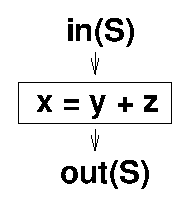
\epsfig{file=in.eps,height=.6in}\end{center}
\begin{small}
avail: x = y + z\\
not avail: x = x + z\\
$out(S) =$ \sout{$gen(S) \cup (in(S) - kill(S))$} - doesn't work\\
$out(S) = (gen(S) \cup in(S)) - kill(S)$\\
$gen(S) = \{ y + z \}$\\
$kill(S) = \{i$ any expr using x $\}$
\end{small}
\end{itemize}
\end{slide}

\begin{slide} {Data Flow Analysis - Available Expressions}
\begin{itemize}
\item[6.] start sets:\\
$out(start) = \{\}$ $\leftarrow$ most safe\\
$out(Si) = \{$ all exprs $\} $ $\leftarrow$ most unsafe \\
\end{itemize}
\end{slide}

\begin{slide} {Data Flow Analysis - Least Fixed Point}
\begin{center}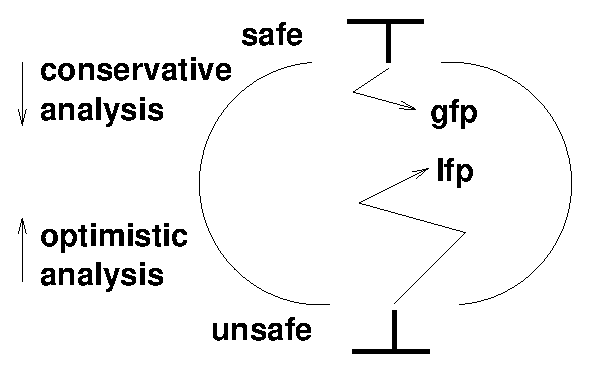
\epsfig{file=lfp.eps,width=3in}\end{center}
\end{slide}

\begin{slide} {Data Flow Analysis - Avail Expr Exercise}
\begin{itemize}
\item switch to Eclipse
\item run Soot on the \texttt{AvailableExpressions.java} sample code
\begin{itemize}
\item right click on file in Package Explorer
\item select Soot - Process Source File - Run Soot ...
\end{itemize}
\item enable Interaction 
\begin{itemize}
\item select General Options - Interactive Mode
\end{itemize}
\end{itemize}
\end{slide}

\begin{slide} {Data Flow Analysis - Avail Expr Exercise}
\begin{itemize}
\item output Jimple
\begin{itemize}
\item select Output Options - Output Format - Jimple File
\end{itemize}
\item enable the Available Expressions Analysis
\begin{itemize}
\item select Phase Options - Jimple Annotation Pack - Available Expressions Tagger
\item check the Enable box
\end{itemize}
\end{itemize}
\end{slide}

\begin{slide} {Data Flow Analysis - Exercise Notes}
\begin{itemize}
\item use the interactive tools to see the generated sets of available expressions 
\item notice this is an optimisitic analysis which starts with full sets everywhere
\end{itemize}
\end{slide}


\begin{slide} {Data Flow Analysis - Avail Expr Exercise - 2}
\begin{itemize}
\item switch to Eclipse
\item run Soot on the \texttt{AvailableExpressions.java} sample code
\begin{itemize}
\item right click on file in Package Explorer
\item select Soot - Process Source File - Run Soot ...
\end{itemize}
\item enable Interaction 
\begin{itemize}
\item select General Options - Interactive Mode
\end{itemize}
\end{itemize}
\end{slide}

\begin{slide} {Data Flow Analysis - Avail Expr Exercise}
\begin{itemize}
\item output Jimple
\begin{itemize}
\item select Output Options - Output Format - Jimple File
\end{itemize}
\item enable the Available Expressions Analysis
\begin{itemize}
\item select Phase Options - Jimple Annotation Pack - Available Expressions Tagger
\item check the Enable box
\item select Pessimistic for analysis kind
\end{itemize}
\end{itemize}
\end{slide}

\begin{slide} {Data Flow Analysis - Exercise Notes}
\begin{itemize}
\item use the interactive tools to see the generated sets of available expressions 
\item notice this is an pessimistic analysis which starts with empty sets everywhere
\item compare this with the optimistic analysis
\end{itemize}
\end{slide}

\begin{slide} {Data Flow Analysis - Very Busy Expressions}
\begin{center}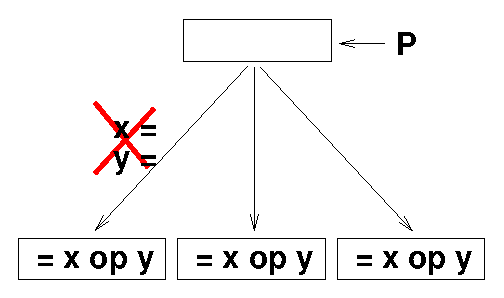
\epsfig{file=verybusy.eps,width=3in}\end{center}
\begin{itemize}
\item $x$ op $y$ is very busy
\end{itemize}
\end{slide}

\begin{slide} {Data Flow Analysis - Very Busy Expressions}
\begin{enumerate}
\item computing: sets of expressions
\item define: an expr e of the form "x op y" is "very busy" at program point p if for all paths from p to the end of the program the expr e is computed and there are no other assignments to x or y from p to the end of the program
\item direction: backwards
\item merge operator: intersection
\end{enumerate}
\end{slide}

\begin{slide} {Data Flow Analysis - Very Busy Expressions}
\begin{itemize}
\item[5.] flow equations:\\
$kill(S) = \{$ any expr involving defs of s$\}$\\
$gen(S) = \{$ x op y$\}$\\
$in(S) = (out(S) - kill(S)) \cup gen(S)$\\
\item[6.] start sets:\\
$in(end) = \{\}$\\
$in(Si) = \{$ all exprs $\}$
\end{itemize}
\end{slide}

\begin{slide} {Data Flow Analysis - Constant Propagation}
Example: \\
\ \\
P1: ((x, 1), (y, ?), (z, 2))\\
P2: ((x, ?), (y, 3), (z, 2))\\
MergePoint: ((x, ?), (y, ?), (z, 2))\\

\end{slide}

\begin{slide} {Data Flow Analysis - Constant Propagation}
\begin{center}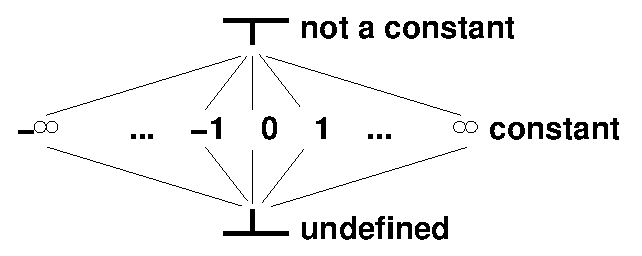
\epsfig{file=constant_lattice.eps,width=3in}\end{center}
\ \\
\ \\
\begin{center}
\begin{tabular}[t]{c|c|c|c} 
$\bowtie$ & $\bot$ & C1 & $\top$ \\ \hline
$\bot$ & $\bot$ & C1 & $\top$ \\ \hline
C2 & C2 & if C1 = C2 C1 else $\top$ & $\top$ \\ \hline
$\top$ & $\top$ & $\top$ & $\top$ 
\end{tabular}
\end{center}
\end{slide}


\end{document}
